\chapter{Data Mining Methods}
\label{ch:mining}

This chapter introduces the data transformation method used in this dissertation.
\section{Remove invalid or missing data}
As a real-world applications of data mining, there are some invalid or missing data in the original data collection. This system should automatically remove invalid data from the raw data and replace missing values with rational information. The rule to handle data is as follows,

\clearpage
\begin{itemize}
	\item Data on holiday. One example is in figure~\ref{fg:invalid_data}, Jan 1, 2016 is New Year Day, and Dec 25, 2015 is Christmas day. There are no transactions on these two days, but in Yahoo Finance, holidays like there are still listed there. Information about Hong Kong holidays are collected from http://www.timeanddate.com/, and after downloading data from Yahoo Finance, the system would automatically remove these holiday transaction data.
	\begin{figure}[h]
		\centering
		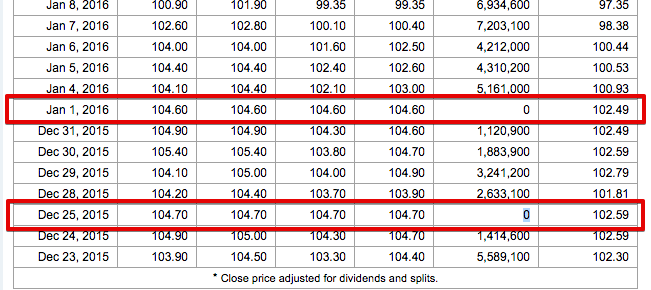
\includegraphics[width=0.9\textwidth]{invalid-data}
		\caption{Example for invalid data}
		\label{fg:invalid_data}
	\end{figure}
\end{itemize}